\documentclass[]{article}
\usepackage[UTF8]{ctex}
\usepackage{amsmath}
\usepackage{graphicx}
\usepackage{ulem}
\newtheorem{theorem}{Theorem}

%opening
\title{保密系统的通信原理\footnote{原始论文信息: Shannon C E . Communication Theory of Secrecy Systems[J]. Bell System Technical Journal, 1949, 28(4):656–715.}}
\author{C. E. Shannon\\
{\small  翻译:李晓峰(cy\_lxf@163.com)}\\
{\small  译文来自于经典文献翻译项目https://gitee.com/uisu/InfSecClaT}\\
{\small 译者单位:北京联合大学智慧城市学院}
}

\usepackage{hyperref} %生产书签

\begin{document}
	
\maketitle
	
	
	\section{引言和概述(INTRODUCTION AND SUMMARY)}
	密码学和保密系统的问题为通信理论提供了一个有趣的应用\footnote{Shannon, C. E., “ A Mathematical Theory of Communication , ”
	Bell System Technical Journal, July 1948 , p. 379 ; Oct. 1948 , p.623 .}。本文提出了一种保密系统理论,该方法在理论层面上,旨在补充密码学以前工作的处理方法\footnote{See , for example , H . F . Gaines , “ Elementary Cryptanalysis , ” or M . Giviergc ,“ Cours de Cryptographic .”}。在那里,对许多标准类型的编码和密码以及破解它们的方法进行了详细的研究。我们将更加关注保密系统的一般数学结构和性质。\par


这个处理方法在某些方面受到限制。首先,一般有三种类型的保密系统:(1)隐蔽系统,包括隐形墨水、在文本中隐藏消息、或密码隐藏在假消息中,或对敌人隐藏消息存在的其他方法;(2)隐私系统,例如语音反转,其中需要特殊设备来恢复信息;(3)“真实”保密系统,其中信息的含义被密码、
代码等隐藏,虽然它的存在并不隐蔽,而且假定敌人拥有拦截和记录传输信号所需的任何特殊设备。我们认为只有第三种类型的隐匿系统是心理上可以接受的技术型的隐私系统。
\par

其次,处理仅限于离散信息的情况,其中要加密的消息由一系列离散符号组成,每个符号从有限的集合中选择。这些符号可以是一种语言中的字母、一种语言中的单词、“量化”语音或视频信号的振幅等,但是主要关注与字母有关的情况。
\par

本文分为三个部分。现在将简要总结主要结果。第一部分论述保密系统的基本数学结构。正如在通信理论中一样,一种语言被认为是由一个随机过程来表示的,这个随机过程根据某种概率系统产生一个离散的符号序列。与语言相关联的是一个特定的参数D,我们称之为语言的冗余。从某种意义上说,D衡量的是语言中的文本在不丢失任何信息的情况下可以缩短多少长度。举个简单的例子,因为在英语单词中u总是跟在q后面,所以u可以省略而不会丢失含义。由于语言的统计结构、某些字母或单词的高频率等原因,英语中可能会有相当多的冗余,冗余在保密系统的研究中至关重要。
\par

保密系统被抽象地定义为一个空间(可能的消息集)到第二个空间(可能的密码集)的一组转换。集合的每个特定变换对应于使用特定密钥进行加密。这些变换被认为是可逆的(非奇异的),因此当密钥已知时,可以进行唯一的解密。\par

在每个转换下,每个密码都有一个与选择此密码概率相关的先验概率。类似地,假设每个可能的消息都有一个相关的先验概率,由潜在的随机过程决定。这些不同密钥和消息的概率实际上是敌方密码分析员对相关选择的先验概率,代表了他对情况的先验知识。\par

要使用保密系统,首先选择一个密钥并将其发送到接收点。密钥的选择决定了构成系统的设备中的特定转换。然后选择一条消息,并将与所选密钥对应的特定转换应用于该消息以生成密文。该密文通过信道传输到接收点,并可能被“敌人”\footnote{“敌人”一词源于军事应用,在密码工作中常用来表示任何可能拦截密码的人。}截获,在接收端,将特定转换的逆运算应用于密文,以恢复原始消息。\par

如果敌人截获了密文(cryptogram),他可以从中计算出可能产生该密文的各种可能消息和密钥的后验概率。这组后验概率构成了他在拦截后对密钥和消息的知识。因此,“知识”被认为是一组与概率相关的命题。后验概率的计算是密码分析的通常解决的问题。
\par

作为这些概念的一个例子,在带有随机密钥的简单替换密码中有26!种转换,对应于26!方式,我们可以替换26个不同的字母。这些选择的可能性是一样的,因此每个都有一个先验概率$1/26$。如果这适用于“普通英语”,密码分析员被假定除了知道是英语文本之外对消息源一无所知,那么N个字母的各种消息的先验概率仅仅是它们在普通英语文本中的相对出现频度。\par

如果敌人在这个系统中截获N个密文字母,他的概率就会改变。如果N足够大(比如50个字母),通常会有一条后验概率几乎为1的消息,而所有其他消息的总概率几乎为零。因此,密文有一个本质上独特的“解法”。对于较小的N(假设N=15),通常会有许多概率相当的消息和密钥,没有一个接近1。在这种情况下,密文有多种“解法”。\par

考虑到一个保密系统将以这种方式表示,作为一组元素到另一组元素的一组转换,自然存在两个组合操作,可以从两个给定系统生成第三个系统。第一组合操作被称为乘积操作,对应于用第一保密系统R对消息进行加密,并用第二系统S对所得密文进行加密,R和S的密钥被独立选择。这个整体操作是一个保密系统,其变换由S变换与R变换的乘积组成。概率是两个变换的概率的乘积。\par

第二种组合操作是“加权加”。\[T=pR+qS \ \ \ \  p+q=1\]

这相当于对系统R或S分别以概率p和q做出初步选择,当这样做时,R或S按照最初定义使用。


研究表明,具有这两种组合运算的保密系统本质上形成了具有单位元素的“线性结合代数”,这是数学家广泛研究的代数变体。


在许多可能的保密系统中,有一种类型具有许多特殊属性。这种类型我们称之为“纯”系统。我们称一个系统是纯的,如果所有密钥的可能性相等,并且如果集合中的任何三种变换$T_i,T_j,T_k$都是乘积	
\[T_iT^{-1}_jT_k\]
也是这个集合上的变换,也就是说,使用任意三个密钥进行加密、解密和加密必须等同于使用某个密钥进行的加密。
	
对于纯密码,证明了所有密钥本质上是等价的,它们都导致相同的后验概率集就,此外,当一个给定的密码被截获时,有一组消息可能产生了这个密码(剩余类),并且这个类中消息的后验概率与先验概率成比例。敌人截获密码获得的所有信息都是剩余类的规范。许多常见密码都是纯的系统,包括使用随机密钥的简单替换。在这种情况下,剩余类由具有与截获密码相同的字母重复模式的所有消息组成。

如果存在具有逆$A^{-1}$的固定变换$A$,则两个系统R和S被定义为“相似”,从而
\[R=AS\]
如果R和S相似,加密结果之间可以建立一对一的对应关系,导致相同的后验概率。两个系统在密码分析上是相同的。


论文的第二部分讨论了“理论保密”(“ theoretical secrecy” )问题。当敌人有无限的时间和人力来分析截获的密码时,系统对密码分析的安全性如何?该问题与存在噪声的通信问题密切相关,为通信问题开发的熵和模糊概念在密码学的这一部分中有直接应用。


“完全保密”(“ Perfect Secrecy ” )的定义是要求系统在密码被敌人截获后,表示各种消息的密码的后验概率与截获前相同消息的先验概率相同。这表明完全保密是可能的,但如果消息数量有限,需要有相同数量的可能密钥。如果消息被认为是以给定的“速率”R(稍后定义)不断生成的,则密钥必须以相同或更高的速率生成。


如果使用具有有限密钥的保密系统,并且截获了N个密文字母,那么对于敌人来说,该密文可能代表一组具有一定概率的消息。随着N的增加,域通常会缩小,直到最终有一个唯一的密文“解”;一个消息的概率基本上是统一的,而所有其他消息实际上都是零。定义了一个量$H(A)$,称为“不确定性”(equivocation,愿意为“含糊其辞”),它以统计方式测量N个字母的平均密文与唯一解的接近程度;也就是说,在截获一个由N个字母组成的密文后,敌人对原始消息的不确定性有多大。推导出了“不确定性”的各种属性,例如,密钥的“不确定性”永远不会随着N的增加而增加,这种“不确定性”是一种理论上的保密指数,理论上,它允许敌人有无限时间分析密码。


确定了称为随机密码的某种理想化类型密码的函数$H(N)$,经过某些修改,该函数可应用于许多实际情况。这提供了一种计算获得保密系统解决方案所需截获材料数量的近似方法。从分析中可以看出,对于普通语言和常用方法密码类型(不是代码)这个“唯一性距离”大约是$H(K)/D$。这里,$H(K)$是一个测量密钥空间“大小”的数字。如果所有密钥都是先验的,那么$H(K)$是可能的密钥数的对数。D是语言的冗余度,并测量语言施加的“统计约束”的数量。简单替换为随机密钥$H(K)$是$log_{10}26!$或大约20,而D(每个字母的十进制数字)在英语中约为0.7。因此,在大约30个字母处出现唯一性。


有可能为“某语言”构造具有有限密钥的保密系统,当$N\rightarrow \inf$时,其不确定性不接近零。在这种情况下,无论截获了多少材料,敌人仍然无法获得密码的唯一解,仍有许多有合理概率的选择,这种系统我们称之为理想系统。在任何语言中都有可能近似这种行为,换言之,可以后退到任意大的$N$使$H(N)$接近零。然而,这种系统有许多缺点,例如密码传输的复杂性和对错误的敏感性。

论文的第三部分涉及“实际保密”(“practical secrecy”)。当截获$N$个字母时,具有相同密钥大小的两个系统可能都是唯一可解的,但在实现该解决方案所需的劳动量上存在很大差异。分析了保密系统的基本弱点。这产生了构建需要大量工作才能解决的系统的方法。最后,讨论了保密系统各种期望质量之间的某种不兼容性。

\begin{center}
	\section*{第一部分\ 保密系统的数学结构(MATHEMATICAL STRUCTURE OF SECRECY SYSTEMS)}
\end{center}

\section{保密系统(SECRECY SYSTEMS)}

作为密码学数学分析的第一步,并以数学上可接受的方式定义我们所说的保密系统。图\ref{Fig:fig1}中显示了一般保密系统的“示意图”。在发送端有两个信息源:消息源和密钥源。密钥源从系统中可能的密钥中产生特定密钥。该密钥通过某种方式发送,消息源产生一条消息(“清除”),该消息被加密,将生成的密文发送给接收端,敌手通过可能的可拦截手段(例如无线电)。在接收端,密文和密钥在解密器中组合以恢复消息。
\par

\begin{figure}[htbp]
	\centering
	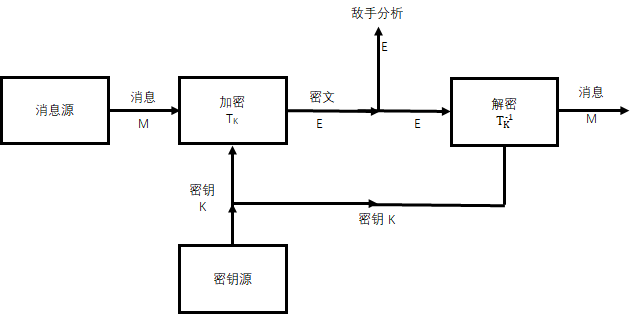
\includegraphics[width=0.8\textwidth]{general-secrecy-system.png}
	\caption{一般保密系统示意图}
	\label{Fig:fig1}
\end{figure}

显然,加密程序执行函数操作。如果$M$是消息,$K4$是密钥,$E$是加密消息或密文,我们有\[E=f(M,K)\],即$E$是$M$和$K$的函数。然而,最好不要将其视为两个变量的函数,而是视为(一个参数)操作或变换族,写为\[E=T_iM.\]
变换$T_i$应用于消息$M$产生密文$E$。索引$i$对应于所使用的特定密钥。

通常,我们将假设只有有限数量的可能密钥,并且每个密钥都具有相关联的概率$p_i$。因此,密钥源由统计过程或设备表示,该统计过程或装置从具有相应概率$p_1,p_2\cdots,p_m$的变换集合$T_1,T_2,\cdots,T_m$中选择一个,同样,我们假定有一个有限多个可能的消息$M_1,M_2,\cdots,M_n$,可能的消息对应的先验概率为$q_1,q_2,\cdots,q_n$,可能消息是正常长度为$N$的英文字母序列,相关概率是这些序列在正常英文文本中出现的相对频率。

在接收端,必须能够恢复$M$,知道$E$和$K$。因此,族中的变换$T_i$必须具有唯一的逆$T^{-1}_i$,使得$T_iT^{-1}_i=I$,$I$即恒等式变换,我们有:\[M=T^{-1}_i E.\]

无论如何,该逆必须对每个$E$唯一存在,该逆可以从具有密钥$i$的M中获得。因此,我们得出了这样的定义:保密系统是一组可能消息到一组密文的唯一可逆变换$T_i$的族,该变换$T_i$具有相关联的概率$p_i$。相反,这种类型的任何一组实体都称为“保密系统”。为了方便起见,可能的消息集称为“消息空间”,可能的密文(cryptgrams)集称为"密文空间"。

如果两个保密系统由相同的变换集$T_i$组成,具有相同的消息和密文空间(范围和域)以及相同的密钥概率,则它们将是相同的。

保密系统可以被机械地视为一台机器,上面有一个或多个控件。一个字母序列,即消息,被输入到机器的输入端,第二个序列出现在输出端。控件的特定设置对应于使用的特定密钥。必须规定一些统计方法,从所有可能的密钥中选择密钥。

为了使问题在数学上易于处理,我们假设敌人知道正在使用的系统。也就是说,他知道变换家族$T_i$和选择各种密钥的概率。可能会有人反对这种假设是不现实的,因为密码分析员通常不知道使用了什么系统,也不知道概率。对于这个反对意见有两个答案:

1.由于我们对什么构成保密系统的广泛定义,这种限制比最初看起来要弱得多。假设密码学者截获了一条消息,并且不知道是否使用了替换、换位或维格纳型(Vigen\`{e}re)密码。 他可以认为消息是由一个系统加密的,其中密钥的一部分是使用这些类型中的某一种类型的规范,下一部分是该类型的特定密钥。这三种不同的可能性被分配概率,依据相应类型密码的加密者的先验概率的最佳估计。


2. 这一假设实际上是密码研究中通常使用的假设。它是悲观的,因此是安全的,但从长远来看是现实的,因为人们必须期望自己的系统最终被发现。因此,即使设计了一个全新的系统,敌人也无法为其分配任何先验概率,在其在没发现的情况下,一个人仍然必须对自己最终的知识抱有期望。(Thus even when an entirely new system is devised , so that the enemy cannot assign any a priori probability to it without discovering it himself , one must still live with the expectation of his eventual knowledge .)

这种情况类似于游戏\footnote{ See von Neumann and Morgenstern	"The Theory of Games" Princeton 1947}理论中的情况,假设对手“发现”正在使用的游戏策略。在这两种情况下,假设都用来清晰地描绘对手的知识。


对我们的保密系统定义的第二个可能的反对意见是,没有考虑到在消息中插入空值和使用多个替代项的常见做法。在这种情况下,给定消息和密钥没有唯一的密文,但加密者可以随意从许多不同的密码中选择。这种情况可以处理,但在现阶段只会增加复杂性,而不会实质上改变任何基本结果。

如果消息是由(1)中所述类型的Markoff过程生成的,以表示信息源,则各种消息的概率由Markoff过程的结构决定。然而,目前,我们希望更全面地了解情况,并将消息仅视为具有相关概率的抽象实体集,不一定由字母序列组成,也不一定由Markoff过程产生。

需要强调的是,在本文中,保密系统不是指一个,而是指一组多个转换。在选择密钥后,只使用其中一个转换,并由此将保密系统定义为语言上的单个转换。然而,敌人,不知道选择了什么密钥,“可能”的密钥对他来说与实际的密钥一样重要。事实上,只有这些其他可能性的存在才使系统具有保密性。由于保密性是我们的基本关心点,我们需要使用上文定义的相当详细的保密系统概念。这种情况,此处可能性和现实一样重要,在游戏策略中经常发生。国际象棋游戏的过程很大程度上受到威胁的控制,而这些威胁并未实施。在某种程度上类似于游戏理论中未实现假设的“虚拟存在”。

可以注意到,在我们的定义下,语言上的单个操作形成了一种退化类型的保密系统————一个只有一个单位概率密钥的系统。这样的系统没有保密性————密码分析员通过应用该变换的逆来发现消息,该变换是系统中唯一的一个,在这种情况下,解密者和密码分析员拥有相同的信息。一般来说,解密者的知识和敌方密码分析者的知识之间的唯一区别是解密者知道正在使用的特定密钥,而密码分析员只知道集合中各种密钥的先验概率。解密的过程是将加密中使用的特定变换的逆应用于密码。密码分析的过程是在只给出密文和各种密钥和信息的先验概率下,试图确定消息(或特定密钥)。

当应用于实际情况时,有许多与保密理论有关的困难问题(difficult epistemological questions),或事实上与任何涉及概率问题(特别是先验概率、贝叶斯定理等)的理论有关。抽象地处理,概率理论可以用现代测量理论方法置于严格的逻辑基础上。\footnote{See J . L . Doob , “ Probability as Measure , ” Annals of Math . Statv . 12 , 1941 , pp .206 - 214 .} \footnote{A . Kolmogoroff ,“ Grundbegriffe der Wahrscheinlichkeits rechnung , ” Ergebnisse der Mathematic , v . 2 , No . 3 ( Berlin 1933 ) .}
然而,当应用于实际情况时,尤其是当涉及“主观”概率和不可重复实验时,存在许多逻辑有效性问题。例如,在这里提出的保密方法中,各种密钥和消息的先验概率被假定为敌方密码学家已知————如何根据其对情况的了解确定其估计是否正确。

我们可以构建“瓮与死”( urn and die)类型的人工密码情况,其中先验概率具有明确含义,这里使用的理想化当然是合适的。在其他情况下,我们可以想象,例如,火星入侵者之间的拦截通信,先验概率可能非常不确定,以至于没有意义。大多数实际的密码情况介于这些限制之间。密码分析师可能愿意将可能的消息分类为“合理”、“可能但不可能”和“不合理”,但觉得更精细的细分没有意义。

幸运的是,在实际情况下,只有密钥和消息的先验概率中的极端错误才会导致重要参数中的重大错误。这是因为消息和密文数量的指数行为,以及采用的对数度量。

\section{系统的表示(REPRESENTATION OP SYSTEMS)}
如上定义的保密系统可以以各种方式表示。如图\ref{Fig:fig2}和图\ref{Fig:fig4}所示,一个便于说明的是线图。可能的消息由左边的点表示,可能的密码由右边的点表示。如果某个密钥,如密钥1,将消息M2转换为密码E4,则M2和E4由标记为1的线连接,以此类推。从每一条可能的消息中,每一个不同的密钥都必须出现一行。如果每一个密码都是这样,我们将说系统是关闭的。

\begin{figure}[htbp]
	\centering
	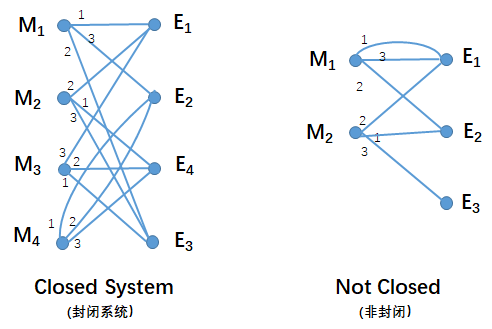
\includegraphics[width=0.8\textwidth]{fig-2.png}
	\caption{简单系统的线条图}
	\label{Fig:fig2}
\end{figure}

描述系统的一种更常见的方法是说明对消息执行的操作,以获取任意密钥的密文。类似地,我们通过描述如何选择密钥或我们知道敌人选择密钥的习惯来隐式地定义各种密钥的概率。消息的概率是由先验知识来隐式确定的,这些知识包括敌人语言习惯,战术情况(这将影响消息的可能内容)以及我们可能拥有的关于密码的任何特殊信息。


\section{保密系统的一些例子(SOME EXAMPLES OF SECRECY SYSTEMS)}

在本节中,将给出一些密码的示例。为了解释的目的,这些示例通常会在本文的其余部分中提及。

\subsection{简单替换密码(Simple Substitution Cipher )}
在这种密码中,消息中的每个字母都被一个固定的替代字母代替,通常也是一个字母。消息:
\[M=m_1 m_2 m_3 m_4\cdots\]
此处$m_1,m_2,\cdots$是连续的字母,变成:
\begin{equation}
\begin{aligned}
	E &=e_1 e_2 e_3 e_4 \cdots \\
	&= f(m_1)f(m_2)f(m_3)f(m_4)\cdots\nonumber
\end{aligned}
\end{equation}
此处$f(m)$函数有逆函数,密钥是字母表的排列(当替代物是字母时),例如$X G U A C D T B F H R S L M Q V Y Z W I E J O K N P$,在这个例子中,第一个字母$X$是$A$的替代物,$G$是$B$的替代物等。


\subsection{换位(固定周期d)(Transposition (Fixed Period d))}
消息被分为长度为$d$的组和应用于第一组的置换,以及应用于第二组的相同置换,等等。置换是密钥,可以由前$d$个整数的置换表示。因此,对于d=5,我们可能有2 3 1 5 4作为置。这意味着:
\begin{equation}
	\begin{aligned}
		&m_1\ m_2\ m_3\ m_4\ m_5 \ m_6\ m_7 \ m_8 \ m_9 \ m_{10} &\cdots \\
		&m_2\ m_3\ m_1\ m_5\ m_4 \ m_7\ m_8 \ m_6 \ m_{10} \ m_9 &\cdots.\nonumber
	\end{aligned}
\end{equation}
两个或多个转置的顺序应用将被称为复合转置(compound transposition)。如果周期为$d_1,\cdots,d_s$,很明显,结果是周期$d$的转置,其中$d$是$d_1,\cdots,d_s$的最小公倍数。

\vspace{1cm}
***********************************************************\par
\textsl{\textbf{译者注:我们用下面一张图来解释加密过程:}}\par
	\begin{figure}[htbp]
		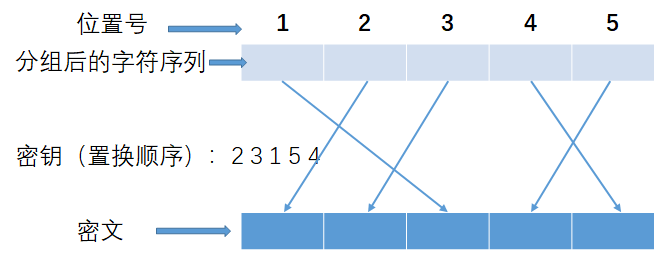
\includegraphics[width=0.8\textwidth]{transpostion-fixedp.png}
	\end{figure}
\par
***********************************************************\par
\vspace{1cm}

\subsection{Vigen\`{e}re及其变种(Vigen\`{e}re and Variations )}
在维格纳密码中,密钥由一系列$d$字母组成。这些字母在消息下方重复书写,并加上两个模26(考虑字母表编号从$A=0到Z=25$),即
\[ e_i = m_i+k_i(mod\ 26) \]
此处$k_i$在索引$i$中为周期$d$,例如,密钥为$G\ A\ H$,我们可以得
\begin{equation}
	\begin{aligned}
	message\ &N\ O\ W\ I\ S\ T\ H\ E\ &\cdots\\
	repeated\ key\ &G\ A\ H\ G\ A\ H\ G\ A\ &\cdots\\
	cryptgram\ &T\ O\ D\ O\ S\ A\ N\ E\ &\cdots\nonumber
	\end{aligned}
\end{equation}

\vspace{1cm}
***********************************************************\par
\textsl{\textbf{译者注:}}\par
上面的计算过程,我们解释一下,首先我们要获得字母对应的数字:\par
\begin{tabular}{|c|c|c|c|c|c|}
	\hline 
	A=0& B=1 & C=2 & D=3 & E=4 & F=5 \\ 
	\hline 
	G=6& H=7 & I=8 & J=9 & K=10 & L=11 \\ 
	\hline 
	M=12& N=13 & O=14 & P=15 & Q=16 & R=17 \\ 
	\hline 
	S=18& T=19 & U=20 & V=21 & W=22 & X=23 \\ 
	\hline 
	Y=24& Z=25 &  &  &  &  \\ 
	\hline 
\end{tabular} 
\par
那么上面的方程就可以写成\par
\begin{equation}
\begin{aligned}
message\ &13\ &14\    &22\ &8\ &18\ &19\ &7\ &4\ &\cdots\\
repeated\ key\ &6\ &0\ &7\ &6\ &0\ &7\   &6\ &0\ &\cdots\\
cryptgram\ &19\ &14\   &3\ &14\ &18\ &0\ &13\ &4\ &\cdots\nonumber
\end{aligned}
\end{equation}

\par
***********************************************************\par

周期1的Vigen\`{e}re被称为凯撒密码。它是一种简单的替换,其中$M$的每个字母在字母表中前进一个固定的量。这个数量是关键,可以是从0到25的任何数字。所谓的波弗特(Beaufort)和变异波弗特(Variant Beaufort)类似于维格纳(Vigen\`{e}re),这两种方式分别通过以下方程加密
\[e_i=k_i-m_i(mod\ 26)\]
和
\[e_i=m_i-k_i(mod\ 26).\]

周期为1的波弗特(Beaufort)密码被称为反向凯撒密码。

两个或多个Vigen\`{e}re按顺序的应用将被称为复合Vigen\`{e}re,公式为
\[e_i=m_i+k_i+l_i+\cdots + s_i(mod\ 26)\]
此处$k_i,l_i,\cdots,s_i$通常有不同的周期,它们和$k_i+l_i+\cdots+s_i$的周期,做为一个符合变换,是各周期的最小公倍数。

当Vigen\`{e}re使用一个没有限制的密钥时,且永不重复,我们有这样一个Vigen\`{e}re系统\footnote{G . S . Vernam ,“ Cipher Printing Telegraph Systems for Secret Wire and Radio Telegraphic Communications , ” Journal American Institute of Electrical Engineers , v . XLV ,pp . 109 - 115 , 1926.}
\[e_i=m_i+k_i(mod\ 26)\]
$k_i$是在$0,1,\cdots,25$中随机和独立选择的。如果密钥是有意义的文本,我们有“运行密钥”( running key)密码。

\subsection{二元图、三元图和N元图替换(Digram , Trigram and N-gram substitution)}

代替字母,我们可以用二元图、三元图等代替。一般的二元图替换需要一个由$26^2$个二元图的排列组成的键。它可以用一个表来表示,其中行对应于二元图中的第一个字母,列对应于第二个字母,表中的条目是替代项(通常也是二元图)。

\subsection{单一混合字母表Vigen\`{e}re(Single Mixed Alphabet Vigen\`{e}re )}
先做一个简单的替换,然后做一个Vigen\`{e}re加密。
\[e_i=f(m_i)+k_i\]
\[m_i=f^{-1}(e_i-k_i)\]
这个系统的“逆”是先做一个Vigen\`{e}re加密,再做一个简单替换。
\[e_i=g(m_i+k_i)\]
\[m_i=g^{-1}(e_i)-k_i\]

\subsection{矩阵系统(Matrix System) \protect\footnote{See L . S . Hill ,“ Cryptography in an Algebraic Alphabet , ” American Math . Monthly ,v. 36 , No. 6 , 1 , 1929, pp. 306 -312 ; also “ Concerning Certain Linear Transformation Apparatus of Cryptography , ” v. 38 , No. 3 , 1931 , pp. 135-154 } }

一种n元代换方法是使用具有逆的矩阵对连续的n元进行运算,假设字母编号为0到25,使其成为代数环的元素。从消息的n元$m_1\ m_2\cdots m_n$,矩阵$a_{ij}$给出n元密文
\[e_i=\sum_{j=1}^{n}a_{ij}m_j\qquad i=1,\cdots,n\]
矩阵$a_{ij}$是密钥,用逆矩阵进行解密。当且仅当行列式$|a_{ij}|$在环中具有逆元素时,逆矩阵将存在。


\subsection{游乐场密码(The Playfair Cipher)}

这是一种特殊类型的数字符号替换,由一个混合的25个字母组成,写在5x5的正方形中。(字母J在密码工作中经常被丢弃————这非常罕见,当它出现时,可以用I代替。)假设密钥正方形如下所示:

\begin{equation}
	\begin{array}{ccccc}
	L &Z &Q &C &P\\
	A &G &N &O &U\\
	R &D &M &I &F\\
	K &Y &H &V &S\\
	X &B &T &E &W \nonumber
	\end{array} 
\end{equation}


例如,数字符号AC的替代物是由A和C定义的矩形的其他两个角上的一对字母,即LO,首先取L,因为它在A之上。如果数字符号与RI在一条水平线上,则使用右边DF的字母;RF变为DR。如果字母在垂直线上,则使用它们下面的字母,因此PS变为UW。如果字母相同,则可以使用空值来分隔它们,或者可以省略一个,等等。

\subsection{多重混合字母替换(Multiple Mixed Alphabet Substitution)}
在这个密码中,有一组按顺序使用的d个简单替换。如果周期d是4,
\[m_1m_2m_3m_4m_5m_6\cdots\]
变成
\[f_1(m_1)f_2(m_2)f_3(m_3)f_4(m_4)f_1(m_5)f_2(m_6)\cdots\]


\subsection{自动密钥密码(Autokey Cipher)}

这是一种Vigen\`{e}re类型的系统,其中消息本身或生成的密文被用作“密钥”,称为自动密钥密码。加密从“启动密钥”(在我们的意义上是整个密钥)开始,并继续使用消息或密文,其长度被启动密钥的长度所取代,如下所示,其中启动密钥是COMET。消息用作“密钥”:
\begin{equation}
	\begin{aligned}
	Message\qquad    &\uwave{SENDSUP}PLIES\cdots \\
	Key\qquad        &\underline{COMET}\uwave{SENDSUP}\cdots \\
	Crytorgram\qquad &USZHLMTCOAYH\cdots \nonumber
	\end{aligned}
\end{equation}

如果用密文做“密钥”则是:\footnote{从保密的角度来看,这个系统是微不足道的,因为除了第一个d字母,敌人拥有整个“密钥”.}
\begin{equation}
	\begin{aligned}
		Message\qquad    &SENDSUPPLIES\cdots \\
		Key\qquad        &\underline{COMET}\uwave{USZHLOH}\cdots \\
		Crytorgram\qquad &\uwave{USZHLOH}OSTS\cdots \nonumber
		\end{aligned}
\end{equation}

\subsection{分馏密码(Fractional Ciphers)}

在这种情况下,每个字母首先被加密为两个或多个字母或数字,这些符号以某种方式混合(例如,通过换位)。然后,结果可能被重新转换为原始字母表。因此,使用混合的25字母表作为密钥,我们可以通过下表将字母转换为两个五位数字:
\begin{center}
	\begin{tabular}{c|c|c|c|c|c}
		
		& 0 & 1 & 2 & 3 & 4 \\ 
		\hline 
		0&L  & Z & Q & C & P \\ 
		\hline 
		1&A  & G & N & O & U \\ 
		\hline 
		2& R & D &M  & I & F \\ 
		\hline 
		3& K & Y & H & V & S \\ 
		\hline 
		4& X & B & T & E & W \\ 
		
	\end{tabular} 
\end{center}


通过查表B转换为41,以此种方式置换后得到的一系列数字,它们被成对地取出来,并翻译回字母。

\subsection{编码(Codes)}
在编码中,单词(有时是音节)被替换为字母组。有时会对结果应用一种或另一种密码。

\section{保密系统的评估(VALUATIONS OF SECRECY SYSTEMS)}

有很多准则可用于估计推荐的保密系统的价值,其中最重要的是下面几个方面:

\subsection{保密程度(Amount of Secrecy)}
有些系统是完美的————敌人拦截任何数量的材料后,情况都不会比以前好。其他系统虽然给了他一些信息,但并不能为拦截的密文提供唯一的“解决方案”。在唯一可解系统中,在实现该解决方案所需努力和所需拦截材料数量方面存在很大差异。

\subsection{密钥大小(Size of Key )}

密钥必须通过不可截获的方式从发送点发送到接收点。有时这一点必须记住。因此,希望密钥尽可能小。

\subsection{加密和解密操作的复杂性(Complexity of Enciphering and Deciphering Operations)}

当然,加密和解密应该尽可能简单。如果人工操作,复杂性会导致时间损失、错误等。如果机械操作,复杂性将导致大型昂贵机器。

\subsection{错误传播(Propagation of Errors)}

在某些类型的密码中,加密或传输中一个字母的错误会导致解密文本中的大量错误。这些错误通过解密操作传播,导致大量信息丢失和频繁需要重复密文。自然希望将这种错误扩展最小化。

\subsection{信息扩展(Expansion of Message)}
在某些类型的保密系统中,消息的大小通过加密过程而增加。在试图通过添加许多空值来淹没消息统计的系统中可以看到这种不期望的效果,或者在使用多个替代的情况下。它也出现在许多“隐藏”( concealment)类型的系统中(通常不是我们定义的保密系统)。

\section{保密系统代数(THE ALGEBRA OF SECRECY SYSTEMS)}
如果我们有两个保密系统$T$和$R$,我们通常用各种办法将他们组合起来形成一个新的保密系统$S$,如果$T,R$有相同的域(消息空间),我们可以形成一个"加权和",
\[S=pT+qR\]
此处$p+q=1$,该操作包括首先用概率$p$和$q$进行初步选择,确定使用$T$和$R$中的哪一个。该选择是S密钥的一部分。确定后,按最初定义使用$T$或$R$。S的全部密钥必须指定使用T和R中的哪一个以及使用T(或R)的密钥。

如果$T$包含变换$T_1,\cdots,T_m$,其选择的概率为$p_1,\cdots,p_m$,$R$包含变换$R_1,\cdots,R_k$,其选择的概率为$q_1,\cdots,q_k$,那么$S=pT+qR$包含变换$T_1,\cdots,T_m,R_1,\cdots,R_k$,其对应的概率分别为$pp_1,pp_2,\cdots,pp_m,qq_1,qq_2,\cdots,qq_k$。

更一般地说,我们可以形成许多系统的总和。
\[S=p_1T+p_2R+\cdots+p_mU \qquad \sum p_i=1\]
我们注意到,任何系统$T$都可以写成固定操作的和
\[T=p_1T_1+p_2T_2+\cdots+p_mT_m\]
$T_i$是对应于密钥选择$i$的确定加密操作,其概率为$p_i$。

组合两个保密系统的第二种方法是采用图\ref{Fig:fig3}中示意性显示的“乘积”。假设$T$和$R$是两个系统,$R$的域(语言(也就是明文)空间)可以用$T$的范围(密文空间)来标识。然后我们可以首先将$T$应用于我们的语言,然后应用$R$生成加密结果。这给出了一个结果运算S,我们将其写成乘积形式
\[S=RT.\]

\begin{figure}[htbp]
	\centering
	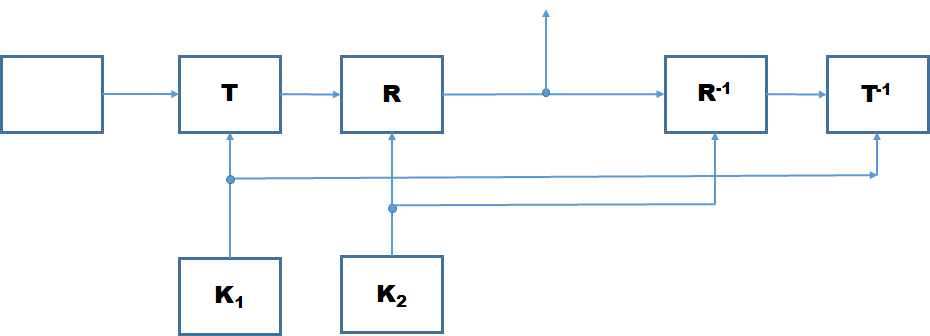
\includegraphics[width=0.8\textwidth]{fig3.png}
	\caption{两个系统的乘积$S=RT$}
	\label{Fig:fig3}
\end{figure}

S的密钥由T和R的两个密钥组成,假设根据它们的原始概率独立地选择。因此,如果$T$的$m$个密钥以概率$p_1\ p_2\cdots p_m$选择,$R$的$n$个密钥具有概率$p'_1\ p'_2\ p'_n$ ,则$S$最多具有$mn$个密钥,概率为$p_ip'_j$。在许多情况下,一些乘积变换$R_iT_j$将是相同的,可以组合在一起,增加它们的概率。

乘积加密经常被使用;例如,一种方法是通过换位或维格纳换位进行替换,或者对文本进行编码,并通过替换、换位、分馏(fractionation )等对结果进行加密。

需要注意的是,乘法通常是不可交换的,(我们不总是有RS=SR),尽管在特殊情况下,如替换和换位,它是可交换的。因为它表示一个运算,所以它是可结合的(associative ),即$R(ST)=(RS)T=RST$。此外,我们还有加法加权结合律定律:
\[p(p'T+q'R)+qS=pp'T+pq'R+qS\]

左右分配律:
\[T(pR+qS)=pTR+qTS\]
\[(pR+qS)T = pRT + qST\]

和
\[p_1T+p_2T+p_3R=(p_1+p_2)T+p_3R\]

应该强调的是,这些加法和乘法的组合运算适用于整个保密系统。两个系统的乘积TR不应与系统$T_iR_j$中变换的乘积混淆,这也经常出现在本文中。前一个$TR$是保密系统,即一组具有相关概率的变换;后者是一个特殊的变换。此外,两个系统的和$pR+qT$是一个系统————两个变换的和没有定义。没有单独的$T_i$和$R_j$可交换(commute)的情况下,系统$T$和$R$也可以是可交换的,例如,如果R是一个给定周期的Beaufort系统,则所有密钥都是相同的,一般我们有,
\[R_iR_j\neq R_jR_i\]
,当然$RR$不取决于其顺序,实际上,$RR=V$具有随机密钥的同一周期的维格纳密码;另一方面,如果两个系统$T$和$R$的单个$T_i$和$R_j$可交换,则整个系统可交换(On the other hand , if the individual Ti and Rj of two systems T and R commute , then the systems commute.)。

一个系统的$M$和$E$空间可以被标识(identified),这是一个非常常见的情况,当字母序列被转换成字母序列时,可以称为内同态(endomorphic)。内同态系统$T$可以被提升到$T^n$的幂。

一个保密系统$T$,其与自身的乘积等于T,即$TT=T$,将被称为幂等的(idempotent)。例如,简单替换、周期$p$的换位、周期p的维格纳密码(每个密钥的可能性相等)都是幂等的。

在固定消息空间中定义的所有自同态保密系统的集合构成“代数变体(algebraic variety)”,即一种代数,使用加法和乘法运算。事实上,我们讨论的加法和乘的性质可以总结如下:\\
\textsl{具有相同消息空间的一组自同态密码以及加权加法和乘法的两个组合运算形成了一个具有单位元素的线性结合代数,除了加权加法中的系数必须是非负的且和为单位之外。}

组合操作为我们提供了从某些类型的保密系统构建许多新类型保密系统的方法,例如给出的示例。我们还可以使用它们来描述密码分析员在试图解决未知类型的密码时面临的情况。事实上,他正在解决下面这种类型的保密系统
\[T=p_1A+p_2B+\cdots+p_rS+p'X \qquad \sum p=1\]
其中$A,B,\cdots,S$是已知类型的密码系统,在这种情况下,$p_i$是它们的先验概率,而$p'X$对应于一种全新未知类型密码的概率。


\section{纯密码和混合密码(PURE AND MIXED CIPHERS)}

某些类型的密码,如简单替换、给定周期的换位、给定周期的维格纳、混合字母维格纳等(每个密钥都具有相同的可能性)相对于密钥具有一定的同质性。无论密钥是什么,加密、解密和解密过程本质上是相同的。这与下面系统形成对比
\[pS+qT\]
其中S是一个简单的替换,T是一个给定周期的换位。在这种情况下,整个系统根据使用的是替换还是换位而改变加密、解密。

这些系统中同质性的原因源于群属性————我们注意到,在上述同质密码的例子中,集合中任何两个变换的乘积$T_iT_j$等于集合中的第三变换$T_k$。另一方面,$T_iS_j$不等于下面密码系统的任何变换:
\[pS+qT\]
它只包含替换和换位,不包含乘积。

因此,我们可以将“pure”密码定义为$T_i$构成的一个群(group)。然而,这将过于限制,因为它要求E空间与M空间相同,即系统是内同态的。分馏换位(fractional transposition)与普通换位一样同质,而不是同态的。正确的定义如下:如果对于每一个$Ti,Tj,Tk$都有一个$T_s$,使得
\[T_iT^{-1}_jT_k=T_s\]
和每个密钥的可能性相等,则密码系统$T$是纯的。否则密码系统是混合的。图\ref{Fig:fig2}的系统是混合的。如果所有密钥的可能性相等,则图\ref{Fig:fig4}是纯的。

\begin{theorem}
	在纯密码中,将消息空间映射到自身的操作$T^{-1}_i T_j$形成一个群,其秩为$m$,即不同密钥的数量。
\end{theorem}

对于$T^{-1}_i T_j T^{-1}_k T_j =  I$,使得每个元素都有一个逆。结合定律是正确的,因为这些运算和群属性遵从:
\[T^{-1}_i T_j T^{-1}_k T_l = T^{-1}_s T_k T^{-1}_k T_l = T^{-1}_s T_l\]
,使用我们的假设,对于某些s,$T^{-1}_i T_j= T^{-1}_s T_k$成立。

当然,$T^{-1}_iT_j$运算意味着用密钥$j$加密消息,然后用密钥$i$解密,这将我们带回到消息空间。如果$T$是自同态的,即$T_i$本身将空间$\Omega_M$映射为自身(如大多数密码的情况,其中消息空间和密码空间都由字母序列组成),并且$T_i$是一个群,并且同样可能,则$T$是纯的,因为\[T_iT^{-1}_jT_k=T_iT_r=T_n.\]

\begin{theorem}
	两个可交换的纯密码系统的乘积是纯的。
\end{theorem}

如果T和R可交换,那么对于每一个i,j,都有一个适当的l,m,使得$T_i R_j= R_l T_m$,并且
\begin{equation}
	\begin{aligned}
		T_iR_j(T_kR_l)^{-1}T_mR_n &=T_i R_j R^{-1}_l T^{-1}_k T_m R_n \\
		                          &=R_u R^{-1}_vR_mT_rT^{-1}_sT_i\\
		                          &=R_hT_v
	\end{aligned}
\end{equation}

然而,交换条件对于乘积是纯密码不是必要的。


只有一个密钥的系统,即单个确定操作$T_1$,是纯的,因为索引的唯一选择是\[T_1T^{-1}_1T_1=T_1.\]
因此,将一般密码扩展为这些简单变换的和也将其显示为纯密码的和。

图\ref{Fig:fig4}所示的纯密码示例揭示了某些属性。消息属于某些子集,我们称之为剩余类(residue classes),可能的密文被划分为相应的剩余类。从一个类中的每个消息到对应类中的每一个密文,至少有条连线,不对应的类之间没有连线。类中的消息数是密钥总数的除数。从消息$M$到相应类中密文“并行”连数等于密钥数除以包含消息(或密文)的类中的消息数。附录中显示了这些对于纯密码一般适用。正式总结,我们有以下定理:

\begin{theorem}\label{source:theorem3}
	在纯系统中,消息可以比分为剩余类集合$C_1,C_2,\cdots,C_8$,密文分成对应的剩余类集合$C'_1,C'_2,\cdots,C'_8$,并且具有以下性质:\\
	(1)消息剩余类是互斥的,共同包含所有可能的消息。类似于文剩余类。\\
	(2)使用任何密钥对$C_i$中的任何消息进行加密会在$C'_i$中生成密文。使用任何密钥解密$C'_i$中的任何密文都会生成$C_i$中的消息。\\
	(3)$C_i$中的消息数,记为$\varphi_i$,等于$C'_i$中的密文数,是密钥数$k$的除数。\\
	(4)$C_i$中的每条消息都可以通过$k/\varphi_i$不同密钥加密为$C'_i$中的一个密文。解密类似。
\end{theorem}

\begin{figure}[htbp]
	\centering
	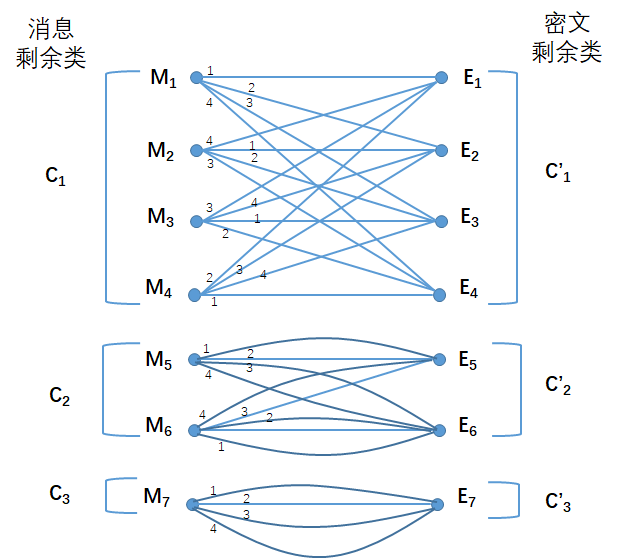
\includegraphics[width=0.6\textwidth]{pure-system.png}
	\caption{"纯"系统}
	\label{Fig:fig4}
\end{figure}

纯密码概念的重要性(以及名称的原因)在于,在纯密码中,所有密钥本质上是相同的。无论对特定消息使用什么密钥,所有消息的后验概率都是相同的。要了解这一点,请注意,应用于同一消息的两个不同密钥会导致同一剩余类中的两个密文,例如$C'_i$。因此,这两个密文可以分别被$\frac{k}{\varphi_i}$个密钥解密为$C_i$中的每个消息,而不是其他可能的消息。所有密钥同样可能是各种消息的后验概率,因此有
\[P_E(M)=\frac{P(M)P_M(E)}{P(E)}= \frac{P(M)P_M(E)}{\sum_M P(M)P_M(E)} =  \frac{P(M)}{P(E)}\]
其中$M$在$C_i$中,$E$在$C'_i$中,并且总和是在$C_i$中的所有消息中。如果$E$和$M$不在相应的剩余类中,则$P_E(M)=0$。类似地,可以显示不同密钥的后验概率值相同,但当使用不同密钥时,这些值与不同密钥相关联。$P_E(K)$的同一组值在密钥之间经历了置换。所以,我们有以下结论:

\begin{theorem}
	在纯系统中,各种消息的后验概率$P_E(M)$独立于所选择的密钥。密钥$P_E(K)$的后验概率在值上相同,但经历具有不同密钥选择的置换。
\end{theorem}

粗略地说,在纯密码中,任何密钥选择都会导致相同的密码分析问题。由于不同的密钥都导致相同剩余类的密文,这意味着相同剩余类中的所有密文在密码分析上是等价的————它们导致相同的消息后验概率,除了置换之外,密钥的概率也相同。

作为一个例子,所有密钥的简单替换都可能是纯密码。对应于给定密文$E$的剩余类是可通过操作$T_jT^{-1}_K E$从E获得的所有密码的集合。在这种情况下,$T_jT^{-1}_k$本身是一个替换,因此$E$上的任何替换都会给出相同剩余类的另一个成员。因此,如果密码是
\[E=X\ C\ P\ P\ G\ C\ F\ Q\]
则
\[E_1=R\ D\ H\ H\ G\ D\ D\ N \]
\[E_2=A\ B\ C\ C\ D\ B\ E\ F \]
等属于同一剩余类。显然,在这种情况下,这些密文本质上是等价的。在使用随机密钥的简单替换中,重要的是字母重复的模式,实际字母是虚拟变量。实际上,我们可以完全省略它们,表明E中的重复模式如下:

\begin{figure}[htbp]
	\centering
	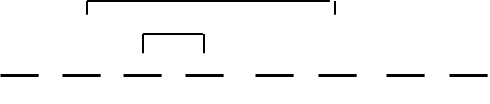
\includegraphics[width=0.6\textwidth]{pattern.png}
\end{figure}

该符号描述了剩余类,但消除了关于类的特定成员的所有信息。因此,它准确地留下了与密码分析相关的信息。这与攻击简单替换密码的一种方法有关————模式词方法。

在凯撒型密码中,只有密文的mod 26这一个差异是重要的。具有相同$\Delta e_i$的两个密文属于同一剩余类。通过写下消息剩余类的26个成员并挑选出有意义的成员的简单过程,就可以破解这个密码。

具有随机密钥的周期为d的维格纳是纯密码的另一个例子。这里,消息剩余类由所有序列组成,这些序列具有与密文相同的一个差异,用于以距离$d$分隔的字母。对于$d=3$,剩余类定义为:
\[m_1-m_4=e_1-e_4\]
\[m_2-m_5=e_2-e_5\]
\[m_3-m_6=e_3-e_6\]
\[m_4-m_7=e_4-e_7\]
\[\cdot\]
\[\cdot\]
\[\cdot\]

此处$E=e_1,e_2,\cdots$是密文$m_1,m_2,\cdots$是在M对应的剩余类的消息。

在具有随机密钥周期为d的换位密码中,剩余类由$e_i$的所有排列组成,其中没有$e_i$移出其长度为d的块,距离$d$处的任何两个$e_i$保持在该距离。这用于破译这些密码,如下所示:密文被写入长度为d的连续块中,一个在另一个下面(d=5):\par
\begin{center}
	\begin{tabular}{c c c c c }
		
		$e_1$& $e_2$ & $e_3$ & $e_4$ & $e_5$ \\ 
		
		$e_6$& $e_7$ & $e_8$ & $e_9$ & $e_{10}$ \\ 
		
		$e_{11}$& $e_{12}$ & $\cdot$ & $\cdot$ & $\cdot$ \\ 
		
		$\cdot$& $\cdot$ & $\cdot$ & $\cdot$ & $\cdot$ \\ 
		
	\end{tabular} 
\end{center}

然后将这些列分割并重新排列,以生成有意义的文本。当列被分割时,剩下的唯一信息是密码的剩余类。

\begin{theorem}
	如果$T$是纯密码系统,那么$T_i T^{-1}_j T= T$,此处$T_iT_j$任意两个$T$的换位变换,相反,如果这对于系统$T$中的任何$T_iT_j$,$T_i T^{-1}_j T= T$,则T是纯的。
\end{theorem}

从纯系统的定义来看,这个定理的第一部分是显而易见的。为了证明第二部分,我们首先注意到,如果$T_i T^{-1}_j T= T$,那么$T_i T^{-1}_j T_s$是T的一个变换。仍然需要证明所有密钥都是等概率的。我们有$T=\sum_{s}p_sT_s$和
\[\sum_{s} p_sT_iT^{-1}_jT_s = \sum_{s}p_sTs.\]

左边项的和在$s=j$时结果为$p_jT_i$。右侧项是$p_iT_i$。由于所有系数都是非负的,因此
\[p_j\leq p_i.\]

当$i,j$互换,相同的讨论也成立,所以有
\[p_j = p_i\]
并且$T$是纯的,$T_iT^{-1}_jT=T$这个条件可以做为纯系统的替代定义。

\section{相似系统(SIMILAR SYSTEMS)}

两个保密系统$R$和$S$将被认为是相似的,如果存在具有逆$A^{-1}$的变换$A$,使得$R=AS$。

这意味着用$R$加密与用$S$加密相同,然后用变换$A$对结果进行操作。如果我们用$R\approx S$ 表示“$R$相似于$S$”,那么很明显$R\approx S$意味着$S\approx R$。$R\approx S$和$S\approx T$也意味着$R\approx T$,并且$R\approx R$。这些可以概括为相似性是一种等价关系。

相似性的密码学意义在于,如果$R\approx S$,则从密码分析的角度来看,$R$和$S$是等价的。事实上,如果密码分析员截获了系统$S$中的密码,他只需对其应用转换$A$,就可以将其转换为系统$R$中的密码。系统$R$中的密码通过应用$A^{-1}$转换为$S$中的密码。如果$R$和$S$应用于相同的语言或消息空间,则生成的密文之间存在一对一的对应关系。对应的密文对所有消息给出相同的后验概率分布。

如果有一种破坏系统$R$的方法,那么任何类似于$R$的系统$S$都可以通过应用操作$A$被破坏。这是一种在实际密码分析中经常使用的设备。

作为一个简单的例子,简单替换(其中替换不是字母而是任意符号)类似于使用字母替换的简单替换。第二个例子是凯撒和反向凯撒型密码。后者在破译时,有时会首先转化为凯撒类型,这可以通过颠倒密文中的字母表来实现。当密钥是随机的时,Vigen\`{e}re、Beaufort和变体Beaufort都是相似的,用密钥$K_1 K_2\cdots K_d$初始化的“自动密钥”密码系统(消息用作“密钥”)类似于Vigen\`{e}re类型,密钥以Mod 26方式交替加和减。在这种情况下,转换$A$是“解密”自动密钥,对启动密钥一系列$d A$操作。

\begin{center}
	\section*{第二部分\ 理论保密(THEORETICAL SECRECY)}
\end{center}

\section{引言(INTRODUCTION)}

\section{完全保密(PERFECT SECRECY)}

\section{不确定性(EQUIVOCATION)}

\section{不确定性属性(PROPERTIES OF EQUIVOCATION)}

\section{双字母语言中简单替换的歧义(EQUIVOCATION FOR SIMPLE SUBSTITUTION ON A TWO LETTER LANGUAGE)}

\section{随机密码的模糊特性(THE EQUIVOCATION CHARACTERISTIC FOR A RANDOM CIPHER)}

\section{标准密码的应用(APPLICATION TO STANDARD CIPHERS)}

\section{密文方案的有效性(VALIDITY OF A CRYPTOGRAM SOLUTION)}

\section{理想保密系统(IDEAL SECRECY SYSTEMS)}

\section{理想保密系统的例子(EXAMPLES OF IDEAL SECRECY SYSTEMS)}

\section{关于模棱两可和冗余的进一步评论(FURTHER REMARKS ON EQUIVOCATION AND REDUNDANCY)}

\section{模糊分布(DISTRIBUTION OF EQUIVOCATION)}

\begin{center}
	%\section*{}
	\Large{第三部分\ 实际保密(PRACTICAL SECRECY)}
\end{center}

\section{工作特点(THE WORK CHARACTERISTIC)}
后来,
\section{密码学解的一般性(GENERALITIES ON THE SOLUTION OF CRYPTOGRAMS)}

\section{统计方法(STATISTICAL METHODS)}


\section{可能词方法(THE PROBABLE WORD METHOD)}

\section{混合变换(MIXING TRANSFORMATIONS)}

\section{$T_k F S_j$类型密码(CIPHERS OF THE TYPE $T_k F S_j$)}

\section{好系统标准的不兼容性(INCOMPATIBILITY OF THE CRITERIA FOR GOOD SYSTEMS)}

\section*{附录(APPENDIX)}
\subsection*{定理\ref{source:theorem3}证明}

\end{document}

